\section{Présentation}
\begin{frame}
\tableofcontents[currentsection]
\end{frame}
\begin{frame}

  \frametitle{Quelles sont les attentes ?}
  
  \centering \huge{Quelles sont les attentes ?}

\end{frame}

\begin{frame}
  \frametitle{Les attentes fonctionnelles}
  \Large{Plusieurs fonctionnalités sont attendues :}
\bigskip
\bigskip
  \begin{columns}[t]
    \begin{column}{.5\textwidth}
      \centering \large Quizz
      \begin{figure}[!h]

        \begin{center}
          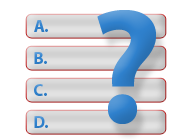
\includegraphics[width = 0.6\textwidth]{presentation/quizz.png}
         \end{center}
      \end{figure}
    \end{column}
    \begin{column}{.5\textwidth}
      \centering \large Jeu(x)
      \begin{figure}[!h]

        \begin{center}
          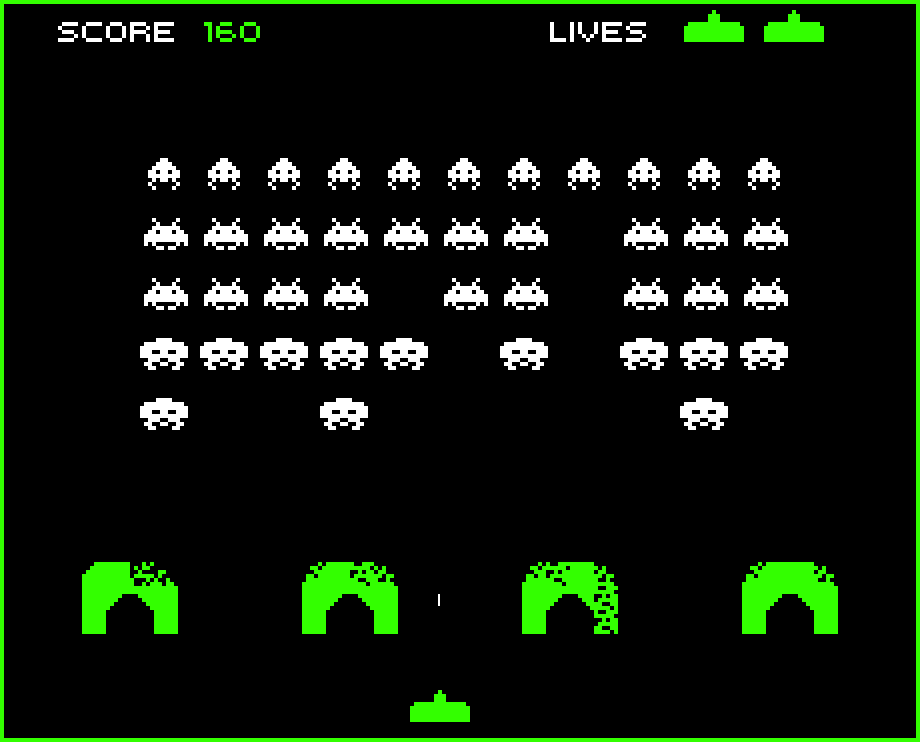
\includegraphics[width = 0.6\textwidth]{presentation/jeu.png}
        \end{center}
      \end{figure}
      
    \end{column}
    
  \end{columns}

\end{frame}

\begin{frame}
  \frametitle{Les attentes fonctionnelles}

  \centering \Large Plusieurs fonctionnalités sont attendues :
\bigskip
  \begin{columns}[t]
    \begin{column}{0.5\textwidth}

      \centering \large Réglages et administration
      \begin{figure}[!h]
        \bigskip
        \begin{center}
          
\includegraphics[width = 0.45\textwidth]{presentation/admin.png}
        \end{center}
      \end{figure}
    \end{column}
    \begin{column}{0.5\textwidth}
      \centering \large Outils musicaux
      \begin{figure}[!h]
        \begin{center}
          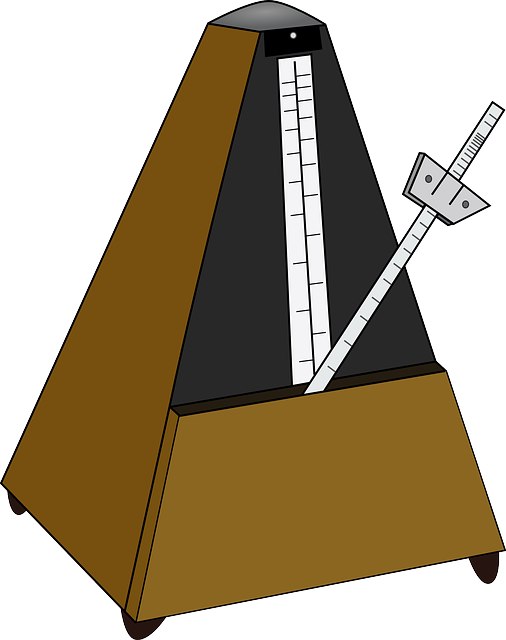
\includegraphics[width = 0.3\textwidth]{presentation/outils1.png}
        \end{center}
      \end{figure}
      
      \begin{figure}[!h]
        \begin{center}
          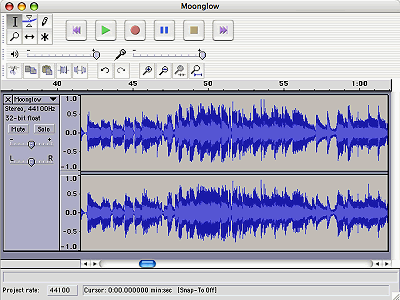
\includegraphics[width = 0.60\textwidth]{presentation/outils2.png}
        \end{center}
      \end{figure}
    \end{column}
    
  \end{columns}
  
\end{frame}


\begin{frame}


  \frametitle{Les autres attentes}
  \large D'autres sont moins fonctionnelles mais nécessaires :
  \bigskip
  \begin{columns}[t]
    \begin{column}{0.5\textwidth}

      \centering \normalsize Logiciel ludique
      \begin{figure}[!h]
        \bigskip
        \begin{center}
          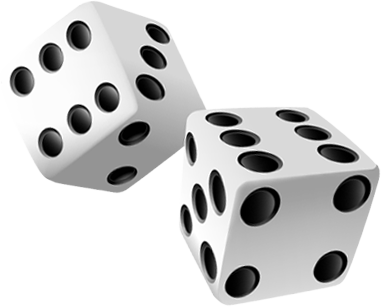
\includegraphics[width = 0.45\textwidth]{presentation/des.png}
        \end{center}
      \end{figure}
    \end{column}
    \begin{column}{0.5\textwidth}
      \centering \normalsize Multi-plateformes
      \begin{figure}[!h]
        \begin{center}
          
\includegraphics[width = 0.30\textwidth]{presentation/windows.png}
        \end{center}
      \end{figure}
      
      \begin{figure}[!h]
        \begin{center}
          
\includegraphics[width = 0.45\textwidth]{presentation/macos.png}
        \end{center}
      \end{figure}
    \end{column}
    
  \end{columns}
\end{frame}

\begin{frame}


  \frametitle{Les autres attentes}
  \large D'autres sont moins fonctionnelles mais nécessaires :
\bigskip
  \begin{columns}[t]
    \begin{column}{0.5\textwidth}

      \centering \normalsize Prise en main intuitive
      \begin{figure}[!h]
        \bigskip
        \begin{center}
          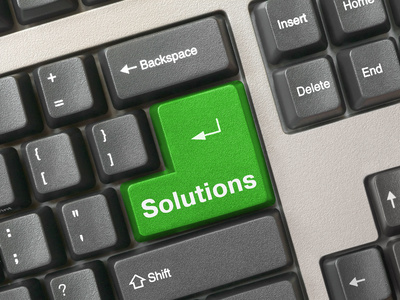
\includegraphics[width = 0.6\textwidth]{presentation/solution.jpg}
        \end{center}
      \end{figure}
    \end{column}
    \begin{column}{0.5\textwidth}
      \centering \normalsize Système évolutif
      \begin{figure}[!h]
        \bigskip
        \begin{center}
          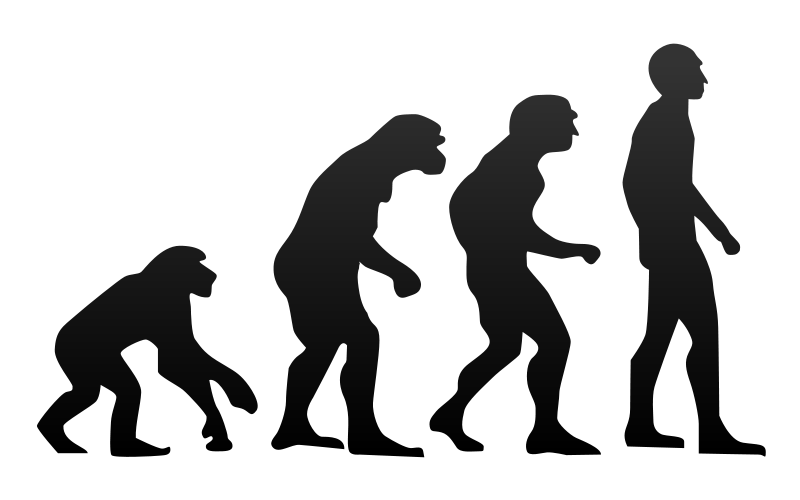
\includegraphics[width = 0.8\textwidth]{presentation/evolution.png}
        \end{center}
      \end{figure}

    \end{column}
    
  \end{columns}
\end{frame}